\section{Le service Web de Yuukou II}

\subsection{Cycle Principal}

\begin{frame}{Cycle principal}
	\begin{block}{Fonctionnement}
		\begin{itemize}
			\item R\'ecup\'eration des donn\'ees Nagios
			\item V\'erifications sur les donn\'ees
			\item Ajout/mise \`a jour/effacement dans la base de donn\'ees
			\begin{itemize}
				\item Ordinateurs
				\item Utilisateurs avec LDAP
				\item Couples ordinateur-utilisateur : archivage d'utilisation
				\item Emplois du temps
			
			\end{itemize}
			
			\item Toutes les minutes

		\end{itemize}

	\end{block}

\end{frame}

%%%%%%%%%%%%%%%%%%%%%%%%%%%%%%%%%

\subsection{Retours client}

\begin{frame}{Retours client}
	\begin{block}{Fonctions publiques}
		\begin{itemize}
			\item Fonctions simples
			\item \'Etats et informations des salles informatiques
			
		\end{itemize}

	\end{block}
	
	\begin{block}{Fonctions priv\'ees}
		\begin{itemize}
			\item Compl\'ements aux fonctions publiques
			\item Gestion du service Web 
			\item Fonctions avanc\'ees
			
		\end{itemize}

	\end{block}

\end{frame}

%%%%%%%%%%%%%%%%%%%%%%%%%%%%%%%%%

\subsection{Fonctionnalit\'es}

\begin{frame}{Fonctionnalit\'es du service Web}
	\begin{block}{S\'ecurisation}
		\begin{itemize}
			\item SSL
			\item Certificats fournis par l'Universit\'e
			
		\end{itemize}

	\end{block}
	
	\begin{block}{G\'en\'eration de statistiques}
		\begin{itemize}
			\item API RRD4J
			\item Graphes d'utilisations des salles informatiques
			
		\end{itemize}

	\end{block}
	
	\begin{block}{Emplois du temps}
		\begin{itemize}
			\item 4 Flux RSS de l'Universit\'e
			\item Correspondance des noms des salles avec le projet
			
		\end{itemize}

	\end{block}
	
\end{frame}

%%%%%%%%%%%%%%%%%%%%%%%%%%%%%%%%%
	
\begin{frame}{Fonctionnalit\'es du service Web}
	\begin{block}{Catalogue logiciels}
		\begin{itemize}
			\item \textit{MediaWiki} pour la \textit{School of Electronics and Computer Science}
			\item Construction des diff\'erents liens
			
		\end{itemize}

	\end{block}
	
	\begin{block}{Gestion des donn\'ees}
		\begin{itemize}
			\item 50 000 \`a 60 000 donn\'ees par mois
			\item D\'eplacement mensuel des donn\'ees d'utilisation
			
		\end{itemize}

	\end{block}

\end{frame}

%%%%%%%%%%%%%%%%%%%%%%%%%%%%%%%%%

\begin{frame}{Utilisation par un client}
	\begin{figure}[h]
		\centering
		\subfloat{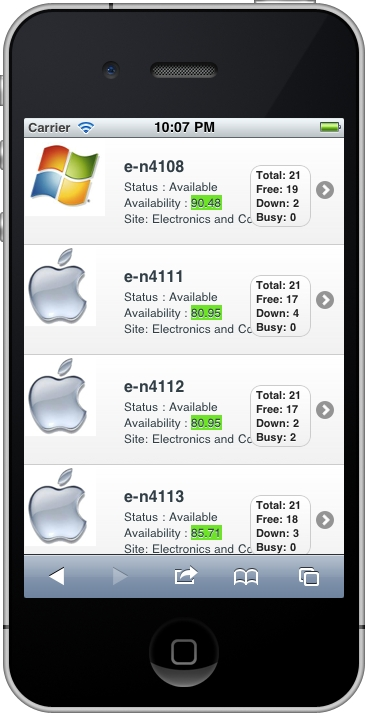
\includegraphics[scale=0.25]{phone.jpg}}
		\qquad
		\subfloat{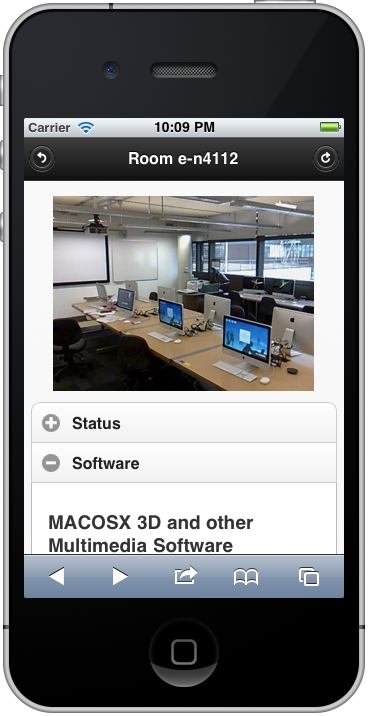
\includegraphics[scale=0.25]{phone1.jpg}}

	\end{figure}
	
\end{frame}

%%%%%%%%%%%%%%%%%%%%%%%%%%%%%%%%%

\subsection{Probl\`emes rencontr\'es}
	
\begin{frame}{Probl\`emes rencontr\'es}
	\begin{block}{Probl\`emes rencontr\'es}
		\begin{itemize}
			\item Manque de connaissances au d\'ebut
			\item Configuration SSL difficile
			\item Normalisation des informations de l'Universit\'e
			
		\end{itemize}

	\end{block}
	
\end{frame}


